%Name: Template of COMP9020 Assignments
%Author:Jack
%Date: 14/08/2017
%Acknowledgement: This template is based on work of Brendan Trinh of UNSW MathSoc 2015
\documentclass[11pt, a4paper]{article}

\usepackage{amsmath} % Improves structure of typed out maths
\usepackage{mathtools} % Improves upon deficiencies of amsmath package
\usepackage{amssymb} % Adds some handy symbols to use.
\usepackage{amsthm} % Adds some neat formulas to use, e.g. \begin{proof} etc.

\usepackage[a4paper]{geometry} % Default page margins can be altered.
\usepackage{microtype} % Improves spacing between letters.
\usepackage{booktabs} % Improves tables. Clan now create without vertical separators.
\usepackage{array} % Includes more options for arrays
\usepackage{paralist} % More flexible use of itemize, enumerate, etc.
\usepackage{graphicx} % Add images to your document
\usepackage{color} % Allows for the use of colours!
\usepackage{cleveref} % Better cross-referencing
\usepackage{hyperref} % For adding hyperlinks
\usepackage{fancyhdr} % Customise headers & footers in document
\usepackage{paralist}

\usepackage{url} % For adding url
\usepackage{multicol} % for multi column
\usepackage[tiny]{titlesec}
\usepackage{enumitem}
\setlist{leftmargin=2mm, topsep=0pt}
\geometry{left=0.8cm, right=0.8cm, top=0.8cm,bottom=0.8cm}
\linespread{0}
\setlength{\parskip}{0\baselineskip}

\begin{document}
\begin{multicols}{3}
% \title{COMP9020 - Review}
% \author{Jack Jiang (z5129432)}
% \date{ 23 October 2017 }
% \maketitle
\graphicspath{{/}}

\section*{Topic 1: Set}
\begin{enumerate}
    \item Floor and ceiling
        \begin{itemize}
            \item $\lfloor \rfloor$: floor
            \item $\lceil \rceil$: ceiling
            \item $\lfloor -X \rfloor = - \lceil X \rceil$
            \item $\lfloor X + t \rfloor = \lfloor X \rfloor + t$ for t $\in$ Z
        \end{itemize}
    \item Divisibility, prime, gcd and lcm
        \begin{itemize}
            \item $m \mid n$: m divides n (m is less)
            \item $n \mid 0$ is true, and $0 \mid n$ is false, except n = 0
            \item prime: $n > 1$ and $1 \mid n$ and $n \mid n$ only
            \item relatively prime: $gcd(m, n) = 1$
            \item gcd: greatest common divisor
            \item lcm: least common multiple
            \item gcd(m, n) * lcm(m, n) = $|m| * |n|$
            \item Euclid's gcd algorithm: for $m > n$, gcd(m, n) = gcd(m-n, n)
        \end{itemize}
    \item Set notation and construction
        \begin{itemize}
            \item symmetric difference:
            \item $A \oplus B = (A \cup B) \setminus (A \cap B)$
            \item $A \oplus B = (A \setminus B) \cup (B \setminus A)$
            \item Subset: $\subseteq$, Proper subset: $\Subset$
            \item Power set: Pow(X) = $\{A: A \subseteq X\}$
            \item Cardinality: $|X|$
            \item Always: $|Pow(X)| = 2^{|X|}$
            \item Set of Numbers: P $\subset$ N $\subset$ Z $\subset$ Q $\subset$ R
            \item De morgan Laws: 
            \item $(A \cup B))^C = A^C \cap B^C$
            \item $(A \cap B))^C = A^C \cup B^C$
            \item Cartesian product:
            \item $A \times B = \{(a,b) | a \in A, b \in B\}$
        \end{itemize}
    \item Formal language
        \begin{itemize}
            \item $\Sigma$: alphabet -- a finite, none empty set
            \item $\lambda$: a empty word
            \item $\Sigma^k$: set of words of length k
            \item $\Sigma^*$: set of all words
            \item $\Sigma^+$: set of none empty words
        \end{itemize}
    \end{enumerate}

\section*{Topic 2: Function Matrix and Relation}
    \begin{enumerate}
        \item Function Definition
            \begin{itemize}
                \item f(x)=y, $f: S \rightarrow T$, $f: x \mapsto y$
                \item every input has an one and only one output
                \item Image: Im(f) = $\{f(x), x \in Dom(f)\}$
                \item Composition: $g \circ f = g(f(x))$ where Im(f) $\subset$ Dom(g)
                \item Identity: $f \circ Id = Id \circ f = f$
            \end{itemize}
        \item Function inverse
            \begin{itemize}
                \item surjective(onto): every output has a related input\\
                    $Im(f) = Codom(f)$
                \item injective(one-to-one): every input has an unique output\\
                    $x \ne y \implies f(x) \ne f(y)$\\
                    $f(x) = f(y) \implies x = y$
                \item bijective: surjective and injective
                \item inverse function: \\
                    $f^{-1}: y \rightarrow x$
                \item inverse image:\\
                    $f^{\Leftarrow}(B) =\{s \in C: f(s) \in B\} \in C$
                \item $f^{-1}(B) = f^{\rightarrow}(B)$
            \end{itemize}
        \item Matrix
            \begin{itemize}
                \item Transpose: $M^{T}$\\
                \item symmetric: $M^T = M$
                \item Product:
                \[
                    \begin{bmatrix}
                        a_{11}  &  a_{12}\\
                        a_{21}  &  a_{22}\\
                    \end{bmatrix}
                    \times
                    \begin{bmatrix}
                        b_{11}  &  b_{12}\\
                        b_{21}  &  b_{22}\\
                    \end{bmatrix}
                    =
                \]
                \[
                    \begin{bmatrix}
                        a_{11}b_{11}+a_{12}b_{21}  &  a_{11}b_{12}+a_{12}b_{22}\\
                        a_{21}b_{21}+a_{22}b_{21}  &  a_{21}b_{12}+a_{22}b_{22}\\
                    \end{bmatrix}
                \]
            \end{itemize}
        \item Relation
            \begin{itemize}
                \item a relation from S to T is a subset of $R \subseteq S \times T$, can be True or False
                \item denote: xRy, R(x, y), x,y $\in$ R
                \item Reflexive: $\forall x \implies xRx$
                \item Anti-reflexive: $\forall x \implies x\not \mathrel{R}x$
                \item Symmetric: $\forall x,y, xRy \implies yRx$
                \item Anti-Symmetric: $\forall x,y, xRy \land yRx \implies x = y$
                \item Transitive: $\forall x,y,z, xRy \land yRz \implies xRz$
                \item a relation CAN NOT be both reflexive and anti-reflexive
                \item a relation CAN be both symmetric and anti-reflexive
            \end{itemize}
        \item Equivalence relation and Order relations
            \begin{itemize}
                \item Equivalence Relation: reflexive, symmetric and Transitive
                \item Partial Order $\preceq$:\\
                    reflexive, antisymmetric, transitive\\
                    lub(least upper bound), $x \in S \land x \succeq a, \forall a \in A$\\
                    glb(greatest lower bound), $x \in S \land x \preceq a, \forall a \in A$\\
                    Lattice: a poset where lub and glb exist for every pair of elements, then they exist for every finite subset
                \item Total Order $\leq$: \\
                    a partial order with Linearity\\
                    arrange every elements in a line $\forall a,b, a \leq b \lor b \leq a$
                \item Well Order: \\
                    a total order with every subset has a least element
            \end{itemize}
        \end{enumerate}

\section*{Topic 3: Graph theory}
    \begin{enumerate}
        \item Definition: a collection of vertices and edges
            \begin{itemize}
                \item Undirected graph: edge = \{v1, v2\}
                \item directed graph: edge = (v1, v2)
                \item denote: v(G) = $|V|$, e(G) = $|E|$
            \end{itemize}
        \item Degree
            \begin{itemize}
                \item Degree: number of edges attached to the vertex
                \item Regular graph: all degree are Equivalence
                \item $\Sigma deg(v) = 2 \times e(G)$\\
                    the degree is always even\\
                    there is an even number of vertices of odd degree
                \item $\Sigma outdeg(v) = \Sigma indeg(v) = e(G)$
            \end{itemize}
        \item Path
            \begin{itemize}
                \item simple path(edge): $e_i \neq e_j$
                \item close path: $v_0 = v_n$
                \item acyclic path(vertex): $v_i \neq v_j$
                \item cycle: acyclic path and close path
                \item acyclic graph: graph contains no cycle
                \item Edge traversal:\\
                    Euler path: path containing every edge exactly once\\
                    iff either it has exactly two vertices of odd degree\\
                    Euler circuit: closed Euler path\\
                    iff all deg(v) is even
                \item Vertex traversal:\\
                    hamiltonian path: visit every vertex exactly once\\
                    hamiltonian circuit: closed hamiltonian path
            \end{itemize}
        \item Connect graph
            \begin{itemize}
                \item connected graph:\\
                    if there is an x-y path $\forall x,y \in V$, denote with k(G)
                \item strongly connected graph(directed):\\
                    each pair of vertices joined by a directed path in both directions
                \item complete graph $K_n$:\\
                    every vertex connected to each other, $\frac {n(n-1)}{2}$ edges.
                \item complete bipartitie graph $K_{m,n}$:\\
                    all vertices form difference parts are connected, vertices from the same part are disconnected.
            \end{itemize}
        \item Tree definitions:
            \begin{itemize}
                \item acyclic, connected
                \item acyclic, $|V_G| = |E_G| + 1$
                \item one simple path between any two vertices
                \item connect, becomes disconnected if any single edge is removed
                \item acyclic, has a cycle is any single edge is added
            \end{itemize}
        \item Graph Isomorphisms
            \begin{itemize}
                \item $ \phi: V_G \rightarrow V_H$ is bijection
                \item $ (x,y) \in E_G$ iff $(\phi(x), \phi(y)) \in E_G$
            \end{itemize}
        \item Colouring and Cliques
            \begin{itemize}
                \item Chromatic number\\
                    $\chi (G):$ the minimum colour
                \item $\chi (Tree) = 2$\\
                    $\chi$ (cycle with even vertices) = 2\\
                    $\chi$ (cycle with odd vertices) = 3
                \item Clique number\\
                    $ \kappa (G) $: the largest complete subgraph
                \item Planar graph: without intersection
                \item a graph is nonplanar then it must contain a subdivision of $K_5$ or $K_{3,3}$
            \end{itemize}
    \end{enumerate}

\section*{Topic 4: Logic}
    \begin{enumerate}
        \item proposition Logic
            \begin{itemize}
                \item statement: a declarative sentence that can be True or False
                \item Well-formed formula(wff)
                \item Connectives: $\lnot p, p \land q, p \lor q, p\implies q$ is a wff.
                \item A implies B: $A \implies B$\\
                    \begin{tabular}{|c|c|c|}
                        \hline
                        A & B & A $\implies$ B\\
                        \hline
                        F & F & T\\
                        \hline
                        F & T & T\\
                        \hline
                        T & F & F\\
                        \hline
                        T & T & T\\
                        \hline
                    \end{tabular}
                \item A unless B: $\lnot B \implies A$
                \item A just in case B: $A \iff B$\\
                    \begin{tabular}{|c|c|c|}
                        \hline
                        A & B & A $\implies$ B\\
                        \hline
                        F & F & T\\
                        \hline
                        F & T & F\\
                        \hline
                        T & F & F\\
                        \hline
                        T & T & T\\
                        \hline
                    \end{tabular}\\
                    $A \iff B$ = $(A \implies B) \lor (B \implies A)$
            \end{itemize}
        \item Logic Equivalence
            \begin{itemize}
                \item $\phi \equiv \varphi$: have the same truth value
                \item De Morgan's Law:\\
                    $ \lnot (p \land q) \equiv \lnot p \lor q$\\
                    $ \lnot (p \lor q) \equiv \lnot p \land q$
            \end{itemize}
        \item formula
            \begin{itemize}
                \item Satisfiable: it can ber true for some assignment of truth value of its basic propositions
                \item Validity Tautology: $\models \phi$ if it is true for all propositions
            \end{itemize}
        \item argument
            \begin{itemize}
                \item Validity, Entailment: an argument is valid if conclusion is true when all premises are true
                \item $\phi_1, \phi_2 \dots \phi_n \models \phi$
            \end{itemize}
        \item Theorem: $\phi \equiv \varphi$ iff $\models (\phi \iff \varphi)$
        \item Proof Method
            \begin{itemize}
                \item Contrapositive: $A \implies B \iff (\lnot B \implies \lnot A)$
                \item Contradiction: $A \iff \lnot A \implies (B \land \lnot B)$
                \item case
                \item substitution
            \end{itemize}
        \item Boolean Function
            \begin{itemize}
                \item             
                \begin{tabular}{|c|c|c|c|}
                    \hline
                    $\land$ & and & $.$ & conjuction\\
                    \hline
                    $\lor$ & or & + & disjunction\\
                    \hline
                    $\lnot$ & not & $\overline p$ & negation\\
                    \hline
                \end{tabular}
                \item CNF: $\prod C = C_1.C_2.C_3 \dots C_n$ 
                \item DNF(prefered): $\sum C = C_1+C_2+C_3 \dots C_n$ 
                \item absortion: $x + xy =x$
                \item combining the opposites: $xy + x\overline y = x$
                \item Demorgan's law
                \item double Negation
                \item
                    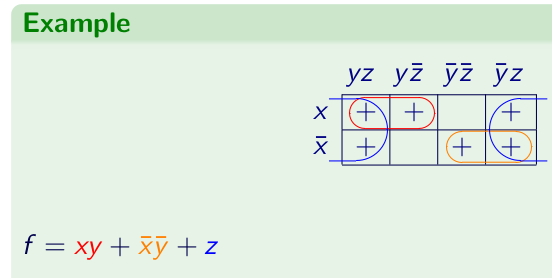
\includegraphics[scale = 0.3]{Kmap}
            \end{itemize}
    \end{enumerate}

\section*{Topic 5: Induction and Recursion}
    \begin{enumerate}
        \item Mathematical Induction
            \begin{itemize}
                \item Base case: first thing is true
                \item Incuctive Hypothesis: Assume sth is true for k, prove that k+1 is true
                \item conclusion
                \item Strong induction: $P(m) \land P(m+1) \land \dots \land P(k) \implies P(k+1)$
                \item F-B induction: $P(k) \implies p(k+1)$ for some k,  $P(k) \implies p(k-1)$ for other k.
            \end{itemize}
        \item $\sum{n} = \frac {(a_1 + a_n)n}{2}$
        \item $\sum{n^2} = \frac{n(n+1)(2n+1)}{6}$
        \item $\prod{n} = \frac {a_1(1-q^n)}{1-q}$
        \item Recursive
            \begin{itemize}
                \item Basis: some initial terms are specified.
                \item Recursive Process: later terms states as functional expressions of earlier terms.
                \item Correctness: if the computation of any later term can be reduced to the initial values give in basis.
            \end{itemize}
    \end{enumerate}

\section*{Topic 6: Programs Analysis}
    \begin{enumerate}
        \item Big O: complexity in terms of input size
            \begin{itemize}
                \item O(f): also be called upper bound\\
                    all function that are asymptotically less than f, which means that $\exists n_0$ for $n > n_0, g < f$
                \item $\Omega(f)$: lower bound
                \item $\Theta(f)$: tight bound
                \item $O(1) < O(logn) < O(n) < O(nlogn) < O(n^2) < O(2^n) < O(n!)$
            \end{itemize}
        \item Master Theorem
            \begin{itemize}
                \item $T(n) = d^a T(f\frac{n}{d}) + \Theta(n^b)$
                \item $O(n^a), a>b$
                \item $O(n^alogn), a=b$
                \item $O(n^b), a<b$
            \end{itemize}
    \end{enumerate}

\section*{Topic 7: Counting and Probability}
    \begin{enumerate}
        \item Counting
            \begin{itemize}
                \item Union rule: for disjoint base sets $|S_1 \cup \dots \cups S_n| = \sum {|S_n|}$
                \item Product rule: $S_1 \times \dots \times S_n = \prod {S_n}$ 
                \item permutation:\\
                    select r items from a size n set, without repetition, order matters
                    $$\Pi (n,r) = \frac {n!}{(n-r)!}$$
                \item combination:\\
                    select r items from a size n set, without repetition, order doesn't matter
                    $$(^{n}_{k})= \frac {n!}{(n-r)!r!}$$
                \item k balls into n box:\\
                    $$(^{n+k-1}_{k})$$
            \end{itemize}
        \item Probability
            \begin{itemize}
                \item Uniform probability distribution:\\
                    each sample has a same probability in sample space $\Omega$\\
                    in a uniform distribution, $P(E) = \frac {|E|}{|\Omega|}$
                \item Event: a collection of outcomes from $\Omega$
                \item Two sets: $|A \cup B| = |A| + |B| - |A \cap B|$
                \item Three sets: $|A \cup B \cup C| = |A| + |B| + |C| - |A \cap B| -|A \cap C| - |B \cap C| + |A \cap B \cap C|$
            \end{itemize}
        \item Conditional Probability and Independence
            \begin{itemize}
                \item Conditional Probability:\\
                    $P(B|A) = \frac {P(A \cap B)}{P(A)}$ for $P(A) \neq 0$
                \item A and B are independent($A \perp B$) iff:\\
                    $P(A \cap B) = P(A)P(B)$\\
                    $P(A|B) = P(A)$ for $P(A) \neq 0$\\
                    $P(B|A) = P(B)$ for $P(B) \neq 0$\\
                    $A \perp B \iff A^C \perp B \iff A \perp B^C \iff A^C \perp B^C$
                \item A and B are mutually exclusive iff $P(A \cap B) = \Phi$
            \end{itemize}
        \item Expectation
            \begin{itemize}
                \item Definition: \\
                    $E(X) = \sum_{k \in Z}{P(X=k)k}$
                \item linearity of expected value:\\
                    $E(X + Y) = E(X) + E(Y)$\\
                    $E(cX) = cE(X)$
                \item Standard deviation: $\varrho$
                \item variance: $\varrho^2\\
                    = E((X - E(X))^2)\\
                    = E(X^2) - E(X)^2$                
            \end{itemize}
    \end{enumerate}


\end{multicols}
\end{document}